\documentclass{article}
\usepackage[utf8]{inputenc}
\usepackage[english]{babel}
\usepackage[font=small,labelfont=bf]{caption}
\usepackage{geometry}
\usepackage{natbib}
\usepackage{pxfonts}
\usepackage{graphicx}
\usepackage{newfloat}
\usepackage{setspace}
\usepackage{hyperref}
\usepackage{lineno}

\newcommand{\argmax}{\mathop{\mathrm{argmax}}\limits}

\newcommand{\topicopt}{S1}
\newcommand{\topics}{S2}
\newcommand{\featureimportance}{S3}
% \newcommand{\listlearning}{S4}
\newcommand{\corrmats}{S4}
\newcommand{\matchmats}{S5}
\newcommand{\wasserstein}{S6}

\doublespacing
\linenumbers


%\title{How is experience transformed into memory?}
%\title{A content-based framework for capturing stimulus and memory dynamics reveals event-like structure in naturalistic episodic recall}
%\title{A content-based model characterizing/describing/representing how experiences and memories unfold over time reveals event-like structure in naturalistic episodic recall}
%\title{A content-based framework describing the temporal dynamics of experiences and memories reveals event-like structure in naturalistic episodic recall}
%\title{A content-based model of how experiences and memories unfold over time reveals event-like structure in naturalistic episodic recall}
\title{A framework for linking dynamic experiences to memories reveals event-like structure in naturalistic episodic recall}

\author{Andrew C. Heusser, Paxton C. Fitzpatrick, and Jeremy R. Manning\\Department of Psychological and Brain Sciences\\Dartmouth College, Hanover, NH 03755, USA\\Corresponding author: jeremy.r.manning@dartmouth.edu}

\bibliographystyle{apa}

\begin{document}
\maketitle

\begin{abstract}
Our life experiences unfold over time and the temporal dynamics of their contents form unique \textit{experience trajectories}.  Within this geometric framework, one can compare the shape of the trajectory formed by an experience to that defined by our later remembering of that experience.  We propose a framework for mapping naturalistic experiences onto geometric spaces that characterize how they unfold over time.  We apply this approach to a naturalistic memory experiment which had participants view and recount a video.  We find that the video and subsequent recall share an event-like structure, and that the shapes of the trajectories formed by participants' recountings were all highly similar to that of the original video. Further, the level of precision that participants' recount the events as well as how distinct their recountings are from other recall events both predict overall subsequent memory performance. Lastly, we identified a network of brain structures that are sensitive to the ``shapes'' of our ongoing experiences, and an overlapping network that is sensitive to how we will later remember those experiences. These result highlight that our dynamic experiences are structured into events in memory, and introduce a novel framework for mapping between dynamic life experiences and their mnemonic counterparts.
\end{abstract}


\section*{Introduction}

What does it mean to \textit{remember} something? In traditional episodic memory experiments \citep[e.g., list-learning or trial-based experiments;][]{Murd62a, Kaha96}, remembering is often cast as a discrete and binary operation: each studied item may be separated from the rest of one's experiences, and that item may be labeled as having been recalled versus forgotten. More nuanced studies might incorporate self-reported confidence measures as a proxy for memory strength, or ask participants to discriminate between ``recollecting'' the (contextual) details of an experience or having a general feeling of ``familiarity'' \citep{Yone02}. Undoubtedly, using well-controlled trial-based experimental designs, the field has amassed a wealth of valuable information regarding human episodic memory.  However, there are fundamental properties of our memories that trial-based experiments are not well suited to capture~\citep[for review also see][]{KoriGold94, HukEtal18}.  First, our memories are continuous, rather than discrete: removing a (naturalistic) event from the context in which it occurs can substantially change its meaning.  Second, the specific language used to describe an experience have little bearing on whether the experience should be considered to have been ``remembered.''  Asking whether the rememberer has precisely reproduced a specific set of words to describe a given experience is nearly orthogonal to whether they were actually able to remember it.  In classic (e.g., list-learning) memory studies, by contrast, counting the number or proportion of precise recalls is often a primary metric of assessing the quality of participants' memories.  Third, one might remember the \textit{essence} (or shape) of an experience but forget (or neglect to recount) particular details.  Capturing the essence of what happened is typically the main ``point'' of recounting a memory to a listener.

How might one go about formally characterizing the shape of an experience, or whether that shape has been recovered by the rememberer?  Any given moment of an experience derives meaning from surrounding moments, as well as from longer-range temporal associations~\citep[e.g., ][]{LernEtal11}.  Therefore, the timecourse describing how an event unfolds is fundamental to its overall meaning.  Further, this hierarchy formed by our subjective experiences at different timescales defines a \textit{context} for each new moment~\citep[e.g., ][]{HowaKaha02, HowaEtal14}, and plays an important role in how we interpret that moment and remember it later~\citep[for review see][]{MannEtal15}.  Our memory systems can then leverage these associations to form predictions that help guide our behaviors~\citep{RangRitc12}.  For example, as we navigate the world, the features of our subjective experiences tend to change gradually (e.g., the room or situation we are in is strongly temporally autocorrelated), allowing us to form stable estimates of our current situation and behave accordingly~\citep{ZackEtal07, ZwaaRadv98}.  

Although our experiences most often change gradually, they also occasionally change suddenly~\citep[e.g., when we walk through a doorway; ][]{RadvZack17}.  Prior research suggests that these sharp transitions (termed \textit{event boundaries}) during an experience help to discretize our experiences into \textit{events}~\citep{RadvZack17, BrunEtal18, HeusEtal18b, ClewDava17, EzzyDava11, DuBrDava13}.  The interplay between the stable (within event) and transient (across event) temporal dynamics of an experience also provides a potential framework for transforming experiences into memories that distill those experiences down to their essence.  For example, prior work has shown that event boundaries can influence how we learn sequences of items~\citep{HeusEtal18b, DuBrDava13}, navigate~\citep{BrunEtal18}, and remember and understand narratives~\citep{ZwaaRadv98, EzzyDava11}. Prior research has implicated the hippocampus and the medial prefrontal cortex as playing a critical role in transforming experiences into stuctured and consolidated memories ~\citep{TompDava17}.

Here we sought to examine how the temporal dynamics of a ``naturalistic'' experience were reflected in participants' later memories of that experience.  We analyzed an open dataset that comprised behavioral and functional Magnetic Resonance Imaging (fMRI) data collected as participants viewed and then verbally recalled an episode of the BBC television series \textit{Sherlock}~\citep{ChenEtal17}.  We developed a computational framework for characterizing the temporal dynamics of the moment-by-moment content of the episode and of participants' verbal recalls.  Specifically, we use topic modeling~\citep{BleiEtal03} to characterize the thematic conceptual (semantic) content present in each moment of the episode and recalls, and we use Hidden Markov Models~\citep{Rabi89, BaldEtal17} to discretize the evolving semantic content into events.  In this way, we cast naturalistic experiences (and recalls of those experiences) as \textit{trajectories} that describe how the experiences evolve over time. Under this framework, successful remembering entails verbally ``traversing'' the topic trajectory of the original episode, thereby reproducing the shape of the original experience.  Comparing the shapes of the topic trajectories of the original episode and of participants' retellings of the episode reveals which aspects of the episode were preserved (or lost) in the translation into memory. 

% NOTE: Can we remove this part? its captured in the abstract
% Using a series of novel memory metrics (introduced here and afforded by our computational framework), we find that the successful memory performance is related to 1) the \textit{precision} with which the participant recounts each event and 2) how \textit{distinctive} each recall event is (relative to the other recalled events). Finally, we identified a network of brain structures whose responses (as participants watched the episode) reflected the shape of the episode, and a second network whose responses reflected how participants would later recount the episode.


\section*{Results}
To characterize the shape of the \textit{Sherlock} episode participants watched and their subsequent recountings of the episode, we used a topic model~\citep{BleiEtal03} to discover the latent thematic content in the video.  Topic models take as inputs a vocabulary of words to consider and a collection of text documents; they return as output two matrices.  The first output is a \textit{topics matrix} whose rows are topics (latent themes) and whose columns correspond to words in the vocabulary. The entries of the topics matrix define how each word in the vocabulary is weighted by each discovered topic.  For example, a detective-themed topic might weight heavily on words like ``crime,'' and ``search.''  The second output is a \textit{topic proportions matrix}, with one row per document and one column per topic.  The topic proportions matrix describes which mix topics is reflected in each document.

\cite{ChenEtal17} collected hand-annotated information about each of 1000 (manually identified) scenes spanning the roughly 45 minute video used in their experiment.  This information included: a brief narrative description of what was happening; whether the scene took place indoors vs. outdoors; names of any characters on the screen; names of any characters who were in focus in the camera shot; names of characters who were speaking; the location where the scene took place; the camera angle (close up, medium, long, etc.); whether or not background music was present; and other similar details (for a full list of annotated features see \textit{Methods}).  We took from these annotations the union of all unique words (excluding stop words, such as ``and,'' ``or,'' ``but,'' etc.) across all features and scenes as the ``vocabulary'' for the topic model.  We then concatenated the sets of words across all features contained in overlapping 50-scene sliding windows, and treated each 50-scene sequence as a single ``document'' for the purposes of fitting the topic model.  Next, we fit a topic model with (up to) $K = 100$ topics to this collection of documents.  We found that 27 unique topics (with non-zero weights) were sufficient to describe the time-varying content of the video (see \textit{Methods}; Figs.~\ref{fig:schematic}, \topics).  Note that our approach is similar in some respects to Dynamic Topic Models~\citep{BleiLaff06}, in that we sought to characterize how the thematic content of the episode evolved over time.  However, whereas Dynamic Topic Models are designed to characterize how the properties of \textit{collections} of documents change over time, our sliding window approach allows us to examine the topic dynamics within a single document (or video).  Specifically, our approach yielded (via the topic proportions matrix) a single \textit{topic vector} for each timepoint of the episode (we set timepoints to match the acquisition times of the 1976 fMRI volumes collected as participants viewed the episode).

\begin{figure}[tp]
\centering
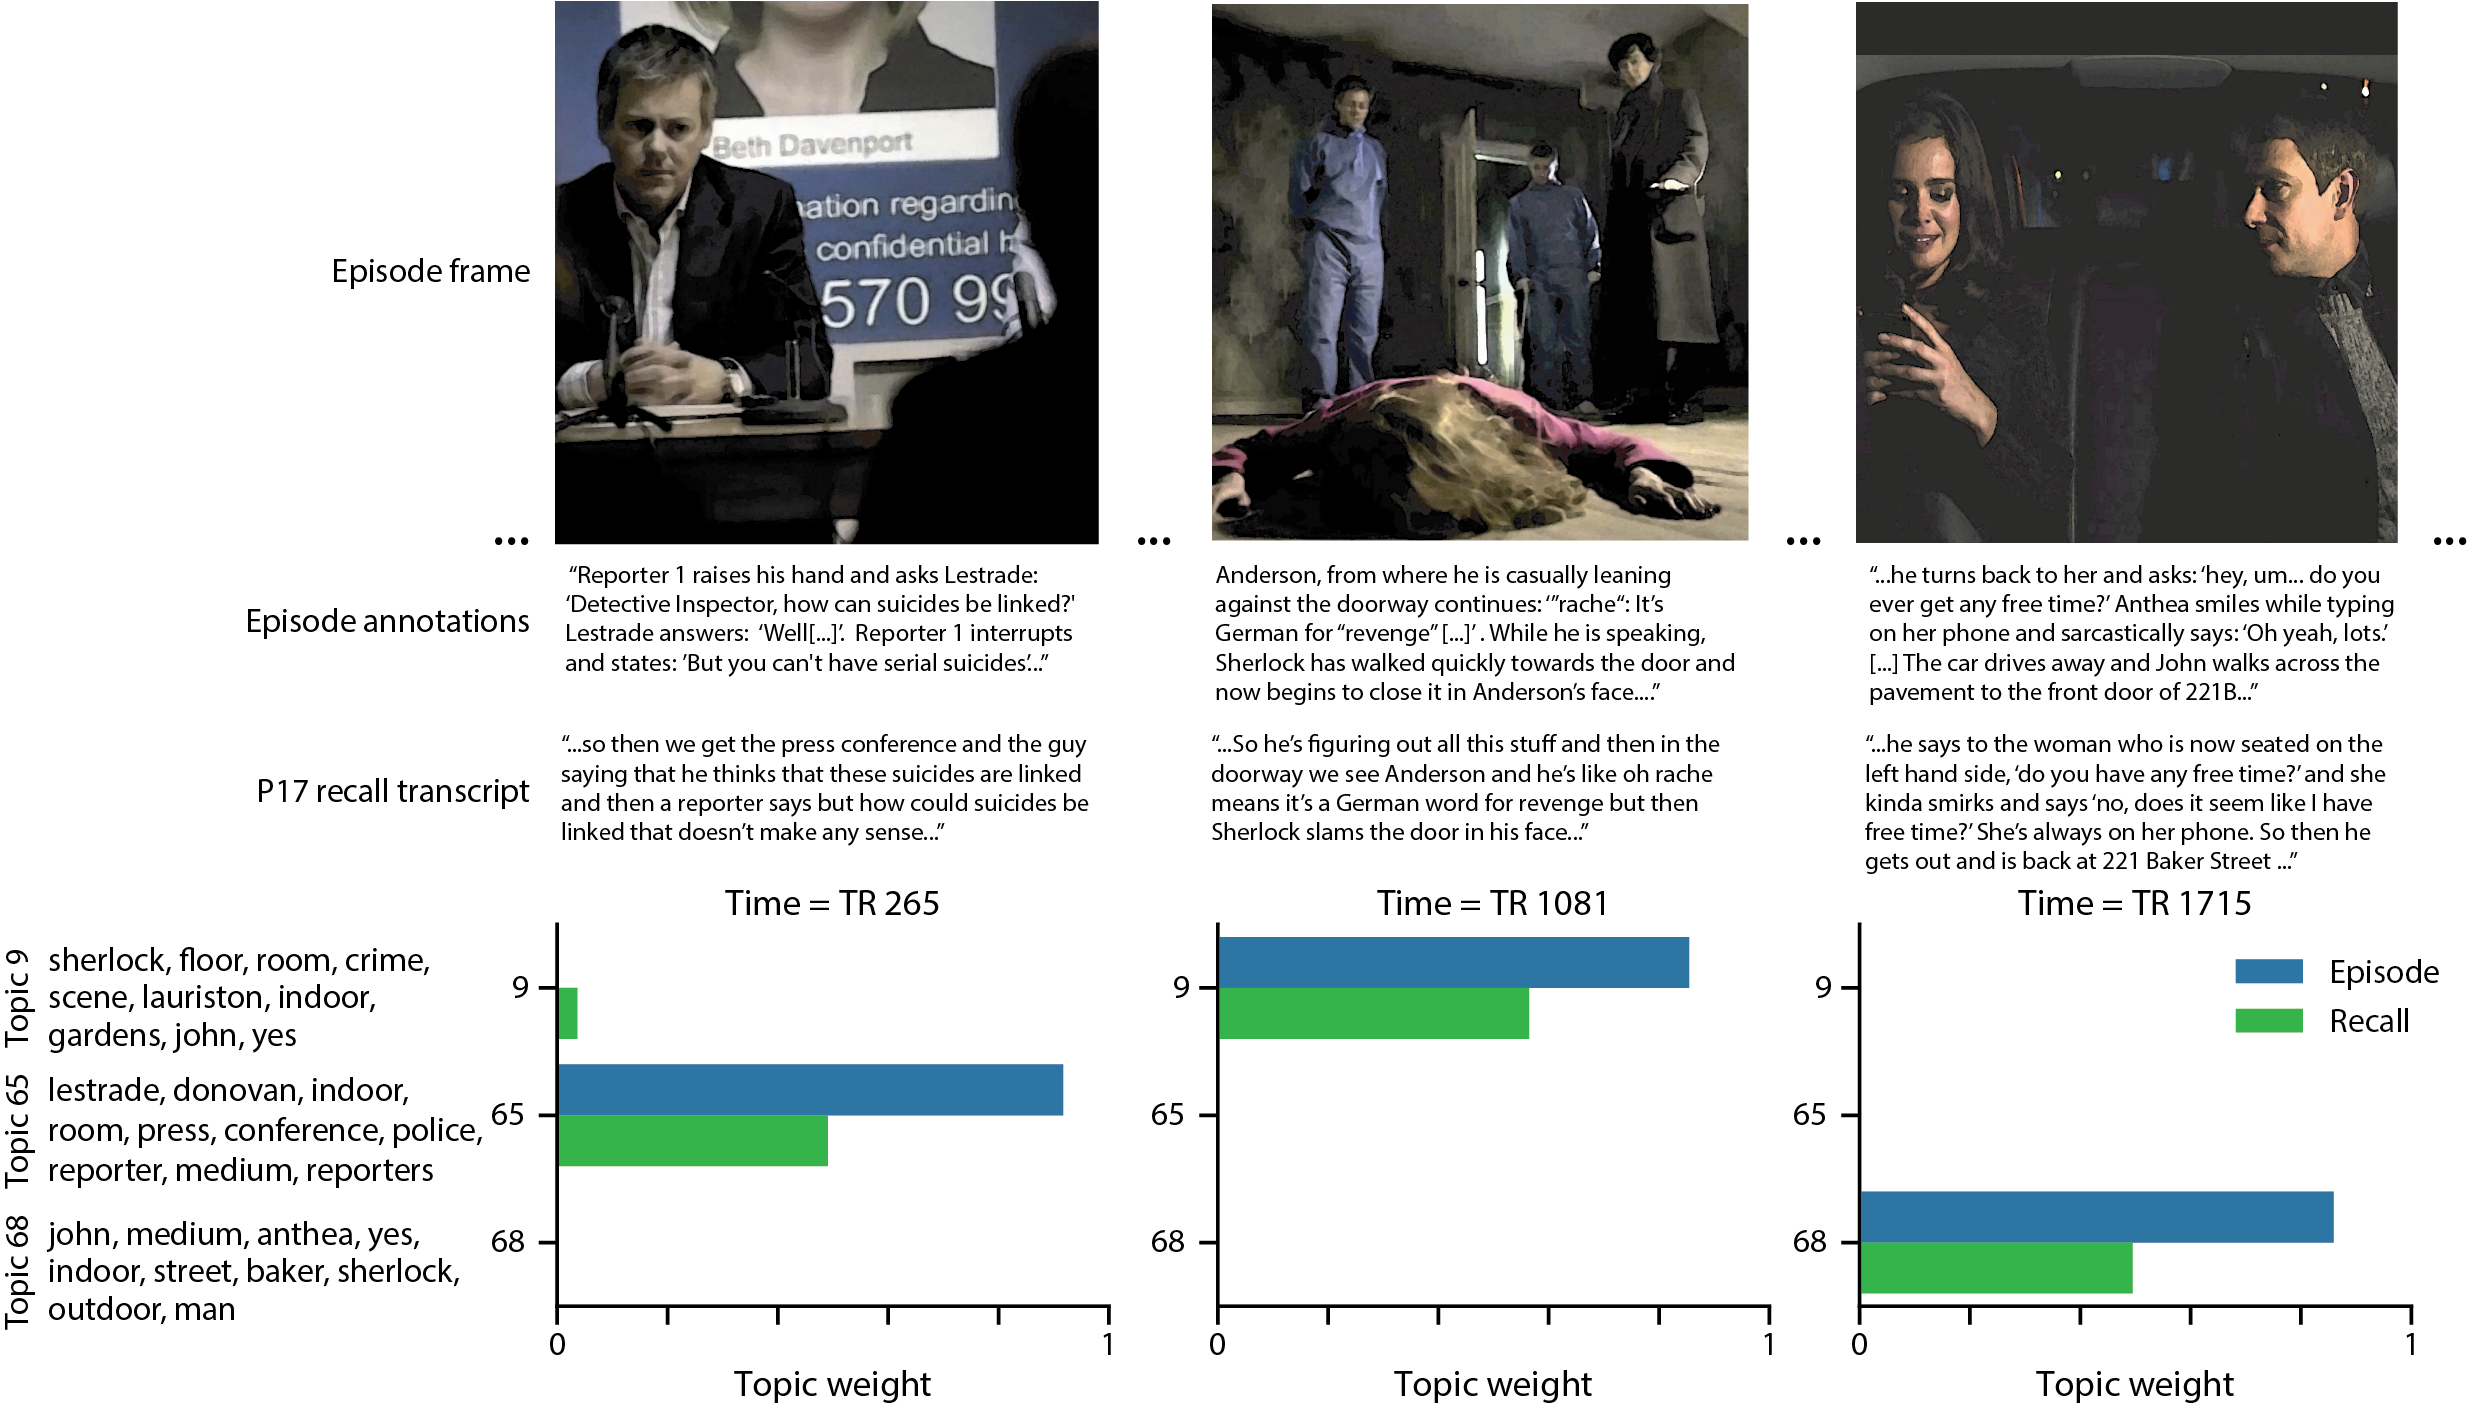
\includegraphics[width=1\textwidth]{figs/schematic}
\caption{\small \textbf{Methods overview.} We used hand-annotated descriptions of each moment of video to fit a topic model.  Three example video frames and their associated descriptions are displayed (top two rows).  Participants later recalled the video (in the third row, we show example recalls of the same three scenes from participant 13).  We used the topic model (fit to the annotations) to estimate topic vectors for each moment of video and each sentence the participants recalled.  Example topic vectors are displayed in the bottom row (blue: video annotations; green: example participant's recalls).  Three topic dimensions are shown (the highest-weighted topics for each of the three example scenes, respectively).  We also show the ten highest-weighted words for each topic.  Figure~\topics~provides a full list of the top 10 words from each of the discovered topics.}
\label{fig:schematic}
\end{figure}

The topics we found were heavily character-focused (e.g., the top-weighted word in each topic was nearly always a character) and could be roughly divided into themes that were primarily Sherlock Holmes-focused (Sherlock is the titular character); primarily John Watson-focused (John is Sherlock's close confidant and assistant); or that involved Sherlock and John interacting (Fig.~\topics).  Several of the topics were highly similar, which we hypothesized might allow us to distinguish between subtle narrative differences (if the distinctions between those overlapping topics were meaningful; also see Fig.~\featureimportance).  The topic vectors for each timepoint were \textit{sparse}, in that only a small number (usually one or two) of topics tended to be ``active'' in any given timepoint (Fig.~\ref{fig:model}A).  Further, the dynamics of the topic activations appeared to exhibit \textit{persistance} (i.e., given that a topic was active in one timepoint, it was likely to be active in the following timepoint) along with \textit{occasional rapid changes} (i.e., occasionally topics would appear to spring into or out of existence).  These two properties of the topic dynamics may be seen in the block diagonal structure of the timepoint-by-timepoint correlation matrix (Fig.~\ref{fig:model}B).  Following \cite{BaldEtal17}, we used a Hidden Markov Model (HMM) to identify the \textit{event boundaries} where the topic activations changed rapidly (i.e., at the boundaries of the blocks in the correlation matrix; event boundaries identified by the HMM are outlined in yellow).  Part of our model fitting procedure required selecting an appropriate number of ``events'' to segment the timeseries into.  We used an optimization procedure to identify the number of events that maximized within-event stability while also minimizing across-event correlations (see \textit{Methods} for additional details).  To create a stable ``summary'' of the video, we computed the average topic vector within each event (Fig.~\ref{fig:model}C).

\begin{figure}[tp]
\centering
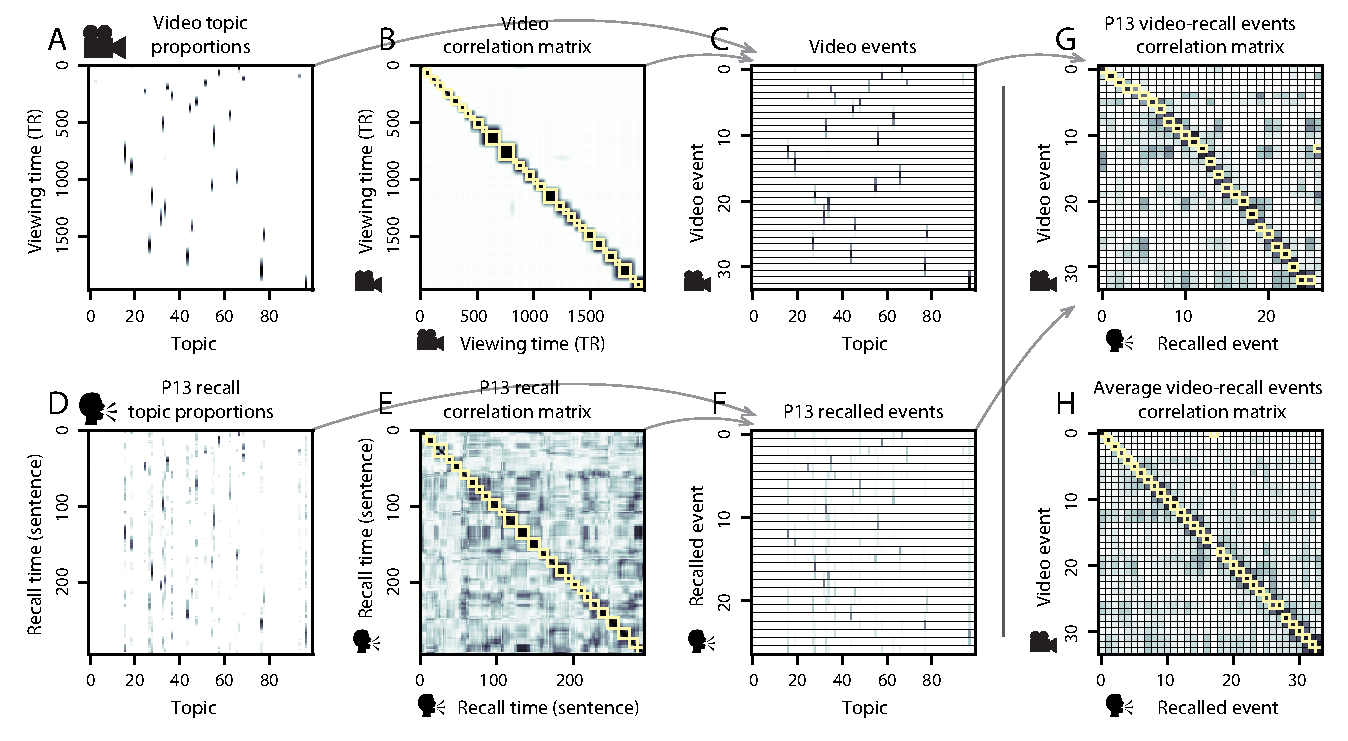
\includegraphics[width=\textwidth]{figs/eventseg}
\caption{\small \textbf{Modelling naturalistic stimuli and recalls.} All panels: darker colors indicate greater values; range: [0, 1].  \textbf{A.} Topic vectors ($K = 100$) for each of the 1976 video timepoints.  \textbf{B.} Timepoint-by-timepoint correlation matrix of the topic vectors displayed in Panel A.  Event boundaries detected by the HMM are denoted in yellow (34 events detected).  \textbf{C.} Average topic vectors for each of the 34 video events. \textbf{D.} Topic vectors for each of 294 sentences spoken by an example participant while recalling the video.  \textbf{E.} Timepoint-by-timepoint correlation matrix of the topic vectors displayed in Panel D. Event boundaries detected by the HMM are denoted in yellow (27 events detected).  \textbf{F.} Average topic vectors for each of the 27 recalled events from the example participant.  \textbf{G.} Correlations between the topic vectors for every pair of video events (Panel C) and recalled events (from the example participant; Panel F).  For similar plots for all participants see Figure~\matchmats.  \textbf{H.} Average correlations between each pair of video events and recalled events (across all 17 participants).  To create the figure, each recalled event was assigned to the video event with the most correlated topic vector (yellow boxes in panels G and H).  The heat maps in each panel were created using \texttt{Seaborn}~\citep{WaskEtal16}.}
\label{fig:model}
\end{figure}

Given that the time-varying content of the video could be segmented cleanly into discrete events, we wondered whether participants' recalls of the video also displayed a similar structure.  We applied the same topic model (already trained on the video annotations) to each participant's recalls.  Analogous to how we analyzed the time-varying content of the video, to obtain similar estimates for participants' recalls, we treated each (overlapping) 10 sentence ``window'' of their transcript as a ``document'' and then computed the most probable mix of topics reflected in each timepoint's sentences.  This yielded, for each participant, a number-of-sentences by number-of-topics topic proportions matrix that characterized how the topics identified in the original video were reflected in the participant's recalls.  Note that an important feature of our approach is that it allows us to compare participant's recalls to events from the original video, despite that different participants may have used different language to describe the same event, and that those descriptions may not match the original annotations.  This is a huge benefit of projecting the video and recalls into a shared ``topic'' space.  An example topic proportions matrix from one participant's recalls is shown in Figure~\ref{fig:model}D.

Although the example participant's recall topic proportions matrix has some visual similarity to the video topic proportions matrix, the time-varying topic proportions for the example participant's recalls are not as sparse as for the video (e.g., compare Figs.~\ref{fig:model}A and D).  Similarly, although there do appear to be periods of stability in the recall topic dynamics (e.g., most topics are active or inactive over contiguous blocks of time), the overall timecourses are not as cleanly delineated as the video topics are.  To examine these patterns in detail, we computed the timepoint-by-timepoint correlation matrix for the example participant's recall topic proportions (Fig.~\ref{fig:model}E).  As in the video correlation matrix (Fig.~\ref{fig:model}B), the example participant's recall correlation matrix has a strong block diagonal structure, indicating that their recalls are discretized into separated events.  As for the video correlation matrix, we can use an HMM, along with the aforementioned number-of-events optimization procedure (also see \textit{Methods}) to determine how many events are reflected in the participant's recalls and where specifically the event boundaries fall (outlined in yellow).  We carried out a similar analysis on all 17 participants' recall topic proportions matrices (Fig.~\corrmats).

Two clear patterns emerged from this set of analyses.  First, although every individual participant's recalls could be segmented into discrete events (i.e., every individual participant's recall correlation matrix exhibited clear block diagonal structure; Fig.~\corrmats), each participant appeared to have a unique \textit{recall resolution}, reflected in the sizes of those blocks.  For example, some participants' recall topic proportions segmented into just a few events (e.g., Participants P1, P4, and P15), while others' recalls segmented into many shorter duration events (e.g., Participants P12, P13, and P17).  This suggests that different participants may be recalling the video with different levels of detail-- e.g., some might touch on just the major plot points, whereas others might attempt to recall every minor scene.  The second clear pattern present in every individual participant's recall correlation matrix is that, unlike in the video correlation matrix, there are substantial off-diagonal correlations in participant's recalls.  Whereas each event in the original video (was largely) separable from the others (Fig.~\ref{fig:model}B), in transforming those separable events into memory participants appear to be integrating \textit{across} different events, blending elements of previously recalled and not-yet-recalled events into each newly recalled event~\citep[Figs.~\ref{fig:model}D, \corrmats; also see][]{MannEtal11, HowaEtal12}.

The above results indicate that both the structure of the original video and participants' recalls of the video exhibit event boundaries that can be identified automatically by characterizing the dynamic content using a shared topic model and segmenting the content into events using HMMs.  Next we asked whether some correspondence might be made between the specific content of the events the participants experienced in the video, and the events they later recalled.  One approach to linking the experienced (video) and recalled events is to label each recalled event as matching the video event with the most similar (i.e., most highly correlated) topic vector (Figs.~\ref{fig:model}G, \matchmats).  This yields a sequence of ``presented'' events from the original video, and a sequence of (potentially differently ordered) ``recalled'' events for each participant.  Analogous to classic list-learning studies, we can then examine participants' recall sequences by asking which events they tended to recall first~\citep[probability of first recall; Fig.~\ref{fig:list-learning}A;][]{WelcBurn24, PostPhil65, AtkiShif68}; how participants most often transition between recalls of the events as a function of the temporal distance between them~\citep[lag-conditional response probability; Fig.~\ref{fig:list-learning}B;][]{Kaha96}; and which events they were likely to remember overall~\citep[serial position recall analyses; Fig.~\ref{fig:list-learning}C;][]{Murd62a}. Interestingly, for 2 of the analyses (probability of first recall and lag-conditional response probability curves) we observe patterns comparable to classic effects from the list-learning literature. Namely, a higher probability of initiating recall with the first event in the sequence (Fig.~\ref{fig:list-learning}A) and a higher probability of transitioning to neighboring events with a forward assymetric bias (Fig.~\ref{fig:list-learning}C). In contrast, we do not observe a pattern comparable to the serial position effect (Fig.~\ref{fig:list-learning}C), but rather we see higher memory for specific events distributed somewhat evenly throughout the video.

% NOTE: Pruning out to tone down the list-learning slander
%In list-learning studies, this set of three analyses may be used to gain a nearly complete view into the sequences of recalls participants made~\citep[e.g., ][]{Kaha12}.  Extending these analyses to apply to naturalistic stimuli and recall~\citep{HeusEtal17b} highlights that, in naturalistic recall, these analyses provide a wholly incomplete picture: they leave out any attempt to quantify participants' abilities to capture the \textit{content} of what occurred in the video-- their only experimental instruction!

\begin{figure}[tp]
  \centering
  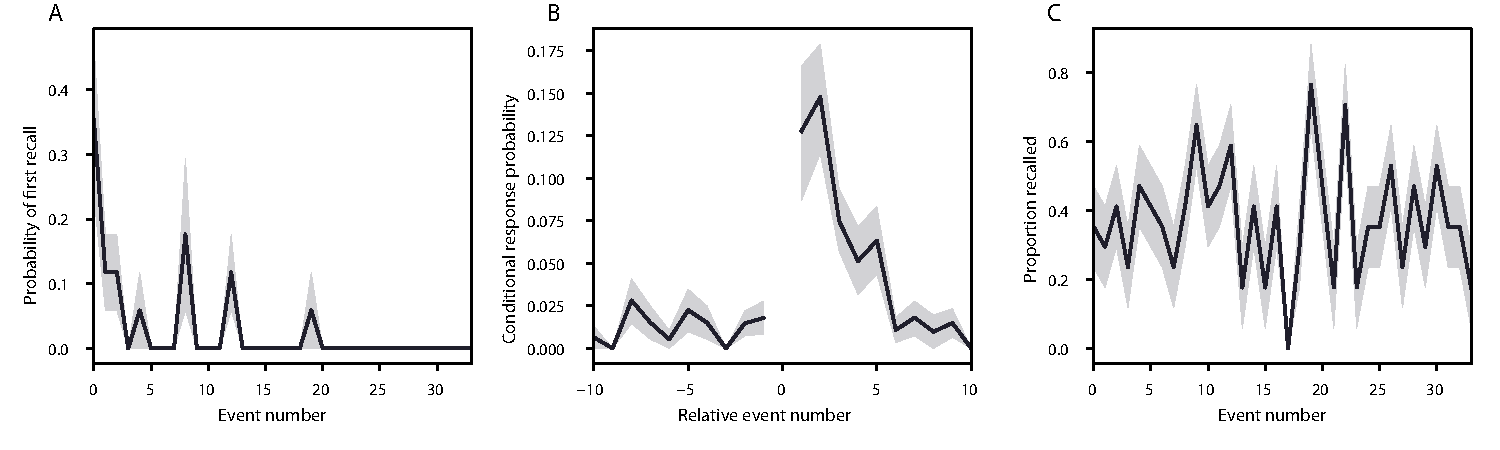
\includegraphics[width=1\textwidth]{figs/list_learning}
  \caption{\small \textbf{Naturalistic extensions of classic list-learning memory analyses.} \textbf{A.} The probability of first recall as a function of the serial position of the event in the video. \textbf{B}.  The probability of recalling each event, conditioned on having most recently recalled the event \textit{lag} events away in the video.  \textbf{C.} The proportion of participants who recalled each event, as a function of the serial position of the events in the video.  All panels: error bars denote bootstrap-estimated standard error of the mean.}
  \label{fig:list-learning}
\end{figure}

Statistical models of memory studies often treat memory recalls as binary (e.g. the item was recalled or not) and independent events.  However, our framework produces a content-based model of individual stimulus events and recall events, allowing for direct quantitative comparison between all stimulus and recall events, as well as between the recall events themselves.  Leveraging this affordance, we introduce 2 novel metrics for quantifying naturalistic memory representations: precision and distinctiveness.  We define precision as the average correlation between each recall event and the maximally correlated video event (Fig.~\ref{fig:precision-distinctiveness}).  Participants whose recall events are more veridical descriptions of what happened in the video event will presumably have higher precision scores. We find that across participants, a higher precision score is correlated to both hand annotated memory performance (Pearson's $r(15) = 0.6, p = 0.011$) as well as the number of recall events (per participant) estimated by our model (Pearson's $r(15) = 0.64, p = 0.005$). A second novel metric we introduce here is the distinctiveness, or the uniqueness of each recall event relative to other recall events. We define distinctiveness as 1 minus the average of all non-matching recall events from the video-recall correlation matrix. We hypothesized that participants who recounted events in a more distinctive way would display better overall memory.  Similar to precision, we find that the more distinct participants recalls are (on average), the more they remembered (hand-annotated memory: Pearson's $r(15) = 0.83, p < 0.001$ and model derived memory: Pearson's $r(15) = 0.71, p = 0.001$).  In summary, using two novel metrics afforded by our approach, we find that participants whose recalls are both more precise and distinct remember more content.

\begin{figure}[tp]
  \centering
  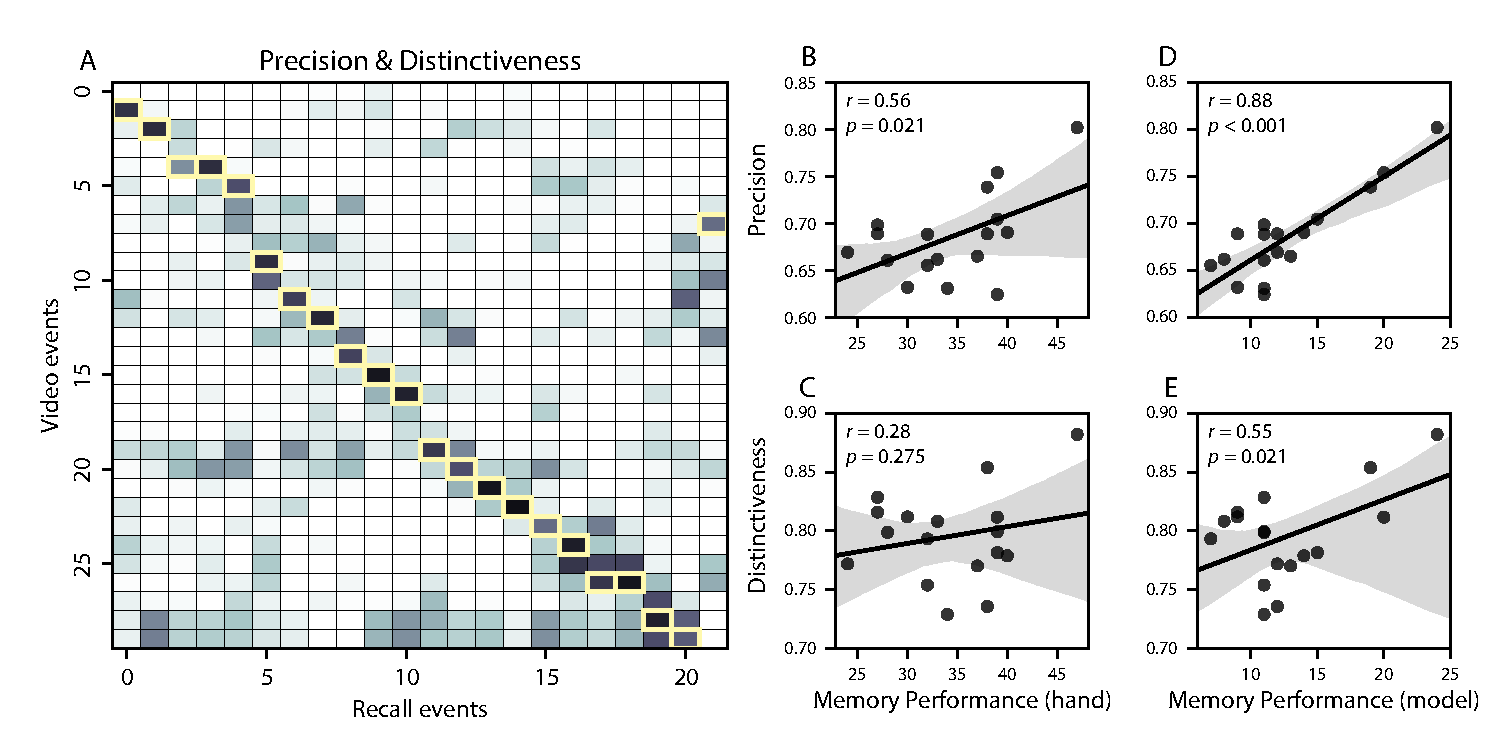
\includegraphics[width=1\textwidth]{figs/precision_distinctiveness}
  \caption{\small \textbf{Novel content-based metrics of naturalistic memory: precision and distinctiveness.} \textbf{A.} A video-recall correlation matrix for a representative participant (17).  The yellow boxes highlight the maximum correlation in each column.  Precision was computed as the average of the maximum correlation in each column.  On the other hand, distinctiveness was defined as the average of everything except for the maximum correlation in each column. \textbf{B.} The (Pearson's) correlation between precision and hand-annotated memory performance. \textbf{C.} The correlation between precision and the number of events recovered by the model ($k$). \textbf{D.} The correlation between distinctiveness and hand-annotated memory performance. \textbf{E.} The correlation between distinctiveness and the number of events recovered by the model ($k$).}
  \label{fig:precision-distinctiveness}
\end{figure}

The dynamic content of the video and participants' recalls is quantified in the corresponding topic proportion matrices.  However, it is difficult to gain deep insights into that content solely by examining the topic proportion matrices (e.g., Figs.~\ref{fig:model}A, D) or the corresponding correlation matrices (Figs.~\ref{fig:model}B, E, \corrmats).  To visualize the time-varying high-dimensional content in a more intuitive way~\citep{HeusEtal18a} we projected the topic proportions matrices onto a two-dimensional space using Uniform Manifold Approximation and Projection~\citep[UMAP; ][]{McInHeal18}.  In this lower-dimensional space, each point represents a single video or recall event, and the distances between the points reflect the distances between the events' associated topic vectors (Fig.~\ref{fig:trajectory}).

\begin{figure}[tp]
\centering
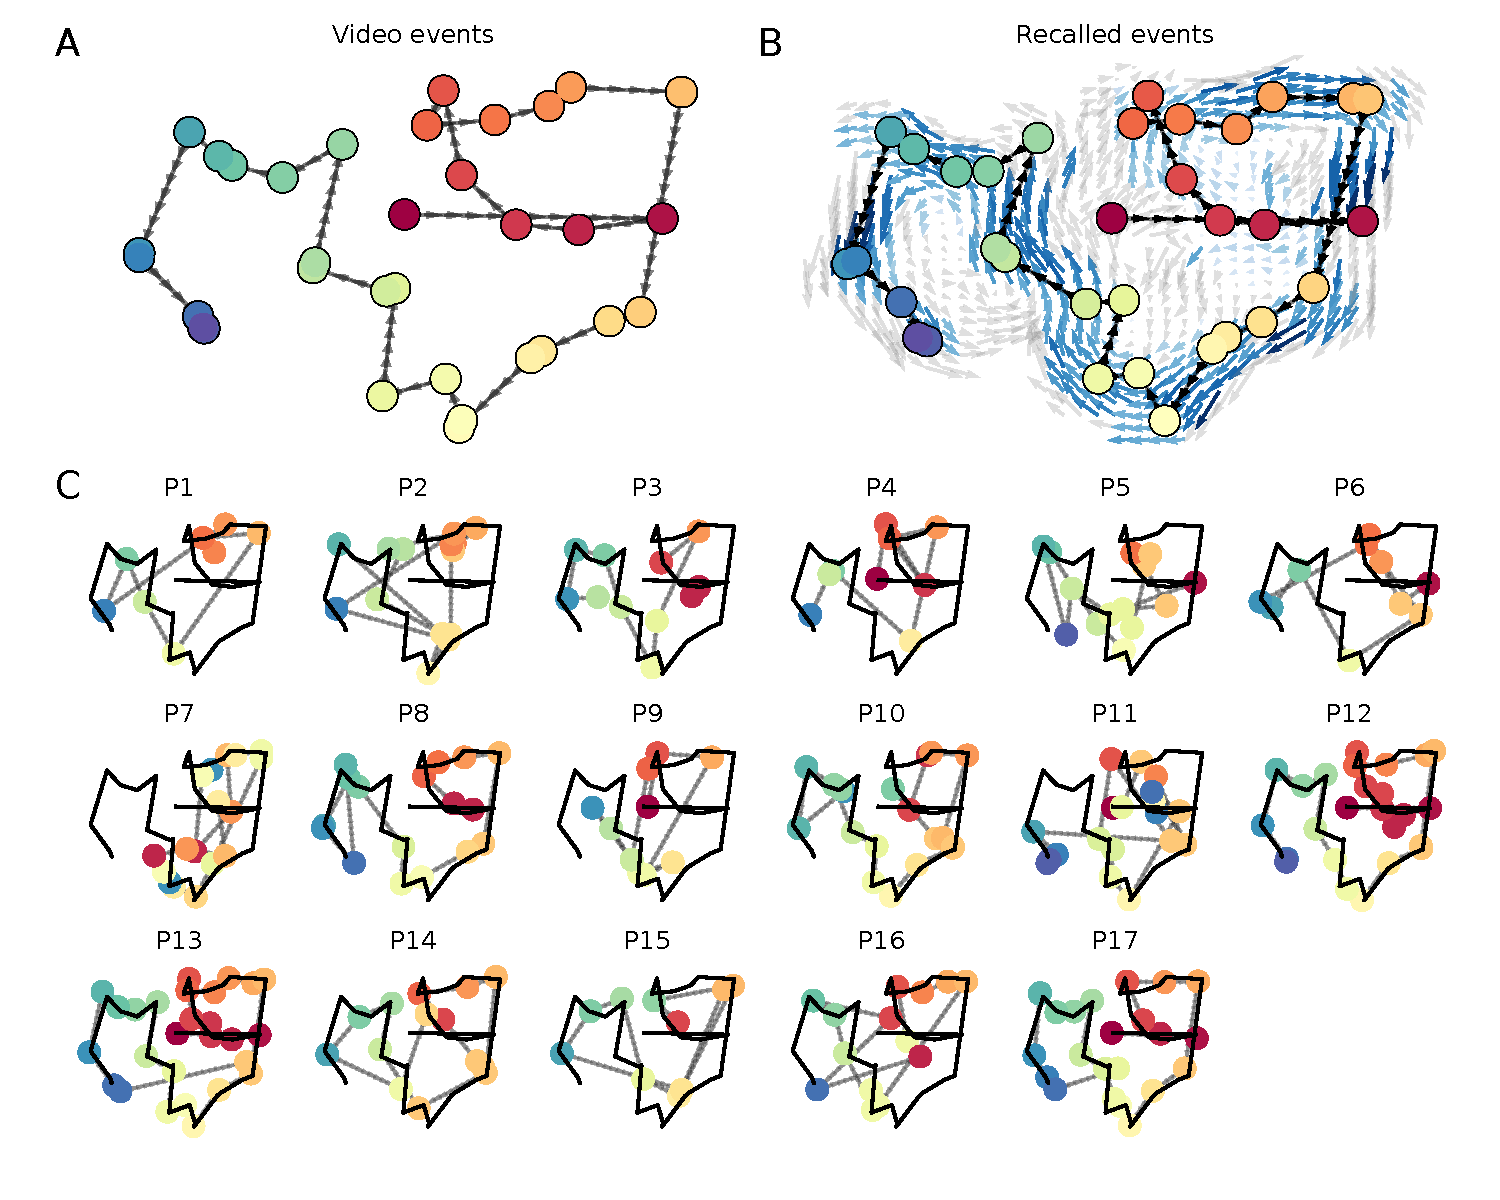
\includegraphics[width=1\textwidth]{figs/trajectory}
\caption{\small \textbf{Trajectories through topic space capture the dynamic content of the video and recalls.}  All panels: the topic proportion matrices have been projected onto a shared two-dimensional space using UMAP.  \textbf{A.} The two-dimensional topic trajectory taken by the episode of \textit{Sherlock}.  Each dot indicates an event identified using the HMM (see \textit{Methods}); the dot colors denote the order of the events (early events are in red; later events are in blue), and the connecting lines indicate the transitions between successive events.  \textbf{B.} The average two-dimensional trajectory captured by participants' recall sequences, with the same format and coloring as the trajectory in Panel A.  To compute the event positions, we matched each recalled event with an event from the original video (see \textit{Results}), and then we averaged the positions of all events with the same label.  The arrows reflect the average transition direction through topic space taken by any participants whose trajectories crossed that part of topic space; blue denotes reliable agreement across participants via a Rayleigh test ($p < 0.05$, corrected).  \textbf{C.} The recall topic trajectories (gray) taken by each individual participant (P1--P17).  The video's trajectory is shown in black for reference.  (Same format and coloring as Panel A.)}
\label{fig:trajectory}
\end{figure}

Visual inspection of the video and recall topic trajectories reveals a striking pattern.  First, the topic trajectory of the video (which reflects its dynamic content; Fig.~\ref{fig:trajectory}A) is captured nearly perfectly by the averaged topic trajectories of participants' recalls (Fig.~\ref{fig:trajectory}B).  To assess the consistency of these recall trajectories across participants, we asked: given that a participant's recall trajectory had entered a particular location in topic space, could the position of their \textit{next} recalled event be predicted reliably?  For each location in topic space, we computed the set of line segments connecting successively recalled events (across all participants) that intersected that location (see \textit{Methods} for additional details).  We then computed (for each location) the distribution of angles formed by the lines defined by those line segments and a fixed reference line (the $x$-axis).  Rayleigh tests revealed the set of locations in topic space at which these across-participant distributions exhibited reliable peaks (blue arrows in Fig.~\ref{fig:trajectory}B reflect significant peaks at $p < 0.05$, corrected).  We observed that the locations traversed by nearly the entire video trajectory exhibited such peaks.  In other words, participants exhibited similar trajectories that also matched the trajectory of the original video (Fig.~\ref{fig:trajectory}C).  This is especially notable when considering the fact that the number of events participants recalled (dots in Fig.~\ref{fig:trajectory}C) varied considerably across people, and that every participant used different words to describe what they had remembered happening in the video.  Differences in the numbers of remembered events appear in participants' trajectories as differences in the sampling resolution along the trajectory.  We note that this framework also provides a means of detangling classic ``proportion recalled'' measures (i.e., the proportion of video events referenced in participants' recalls) from participants' abilities to recapitulate the full shape of the original video (i.e., the similarity in the shape of the original video trajectory and that defined by each participant's recounting of the video).

Because our analysis framework projects the dynamic video content and participants' recalls onto a shared topic space, and because the dimensions of that space are known (i.e., each topic dimension is a set of weights over words in the vocabulary; Fig.~\topics), we can examine the topic trajectories to understand which specific content was remembered well (or poorly).  For each video event, we can ask: what was the average correlation (across participants) between the video event's topic vector and the closest matching recall event topic vectors from each participant? This yields a single correlation coefficient for each video event, describing how closely participants' recalls of the event tended to reliably capture its content (Fig.~\ref{fig:topics}A).  (We also examined how different comparisons between each video event's topic vector and the corresponding recall event topic vectors related to hand-annotated characterizations of memory performance; see \textit{Supporting Information}).  Given this summary of which events were recalled reliably (or not), we next asked whether the better-remembered or worse-remembered events tended to reflect particular topics.  We computed a weighted average of the topic vectors for each video event, where the weights reflected how reliably each event was recalled.  To visualize the result, we created a ``wordle'' image~\citep{MuelEtal18} where words weighted more heavily by better-remembered topics appear in a larger font (Fig.~\ref{fig:topics}B, green box).  Events that reflected topics weighting heavily on characters like ``Sherlock'' and ``John'' (i.e., the main characters) and locations like ``221b Baker Street'' (i.e., a major recurring location and the address of the flat that Sherlock and John share) were best remembered.  An analogous analysis revealed which themes were poorly remembered.  Here in computing the weighted average over events' topic vectors we weighted each event in \textit{inverse} proportion to how well it was remembered (Fig.~\ref{fig:topics}B, red box).  This revealed that events with relatively minor characters such as ``Mike,'' ``Jeffrey,'' and ``Molly,'' as well as less-integral plot locations (e.g., ``hospital'' and ``office'') were least well-remembered.  This suggests that what is retained in memory are the major plot elements (i.e., the overall shape of what happened), whereas the more minor details are prone to pruning.

In addition to constructing overall summaries, assessing the video and recall topic vectors from individual recalls can provide further insights.  Specifically, for any given event we can construct two wordles: one from the original video event's topic vector, and a second from the average topic vectors produced by all participants' recalls of that event.  We can then examine those wordles visually to gain an intuition for which aspects of the video event were recapitulated in participants' recalls of that event.  Several example wordles are displayed in Figure~\ref{fig:topics}C (wordles from the three best-remembered events are circled in green; wordles from the three worst-remembered events are circled in red).  Using wordles to visually compare the topical content of each video event and the (average) corresponding recall event reveals the specific content from the specific events that is reliably retained in the transformation into memory (green events) or not (red events).

\begin{figure}[tp]
\centering
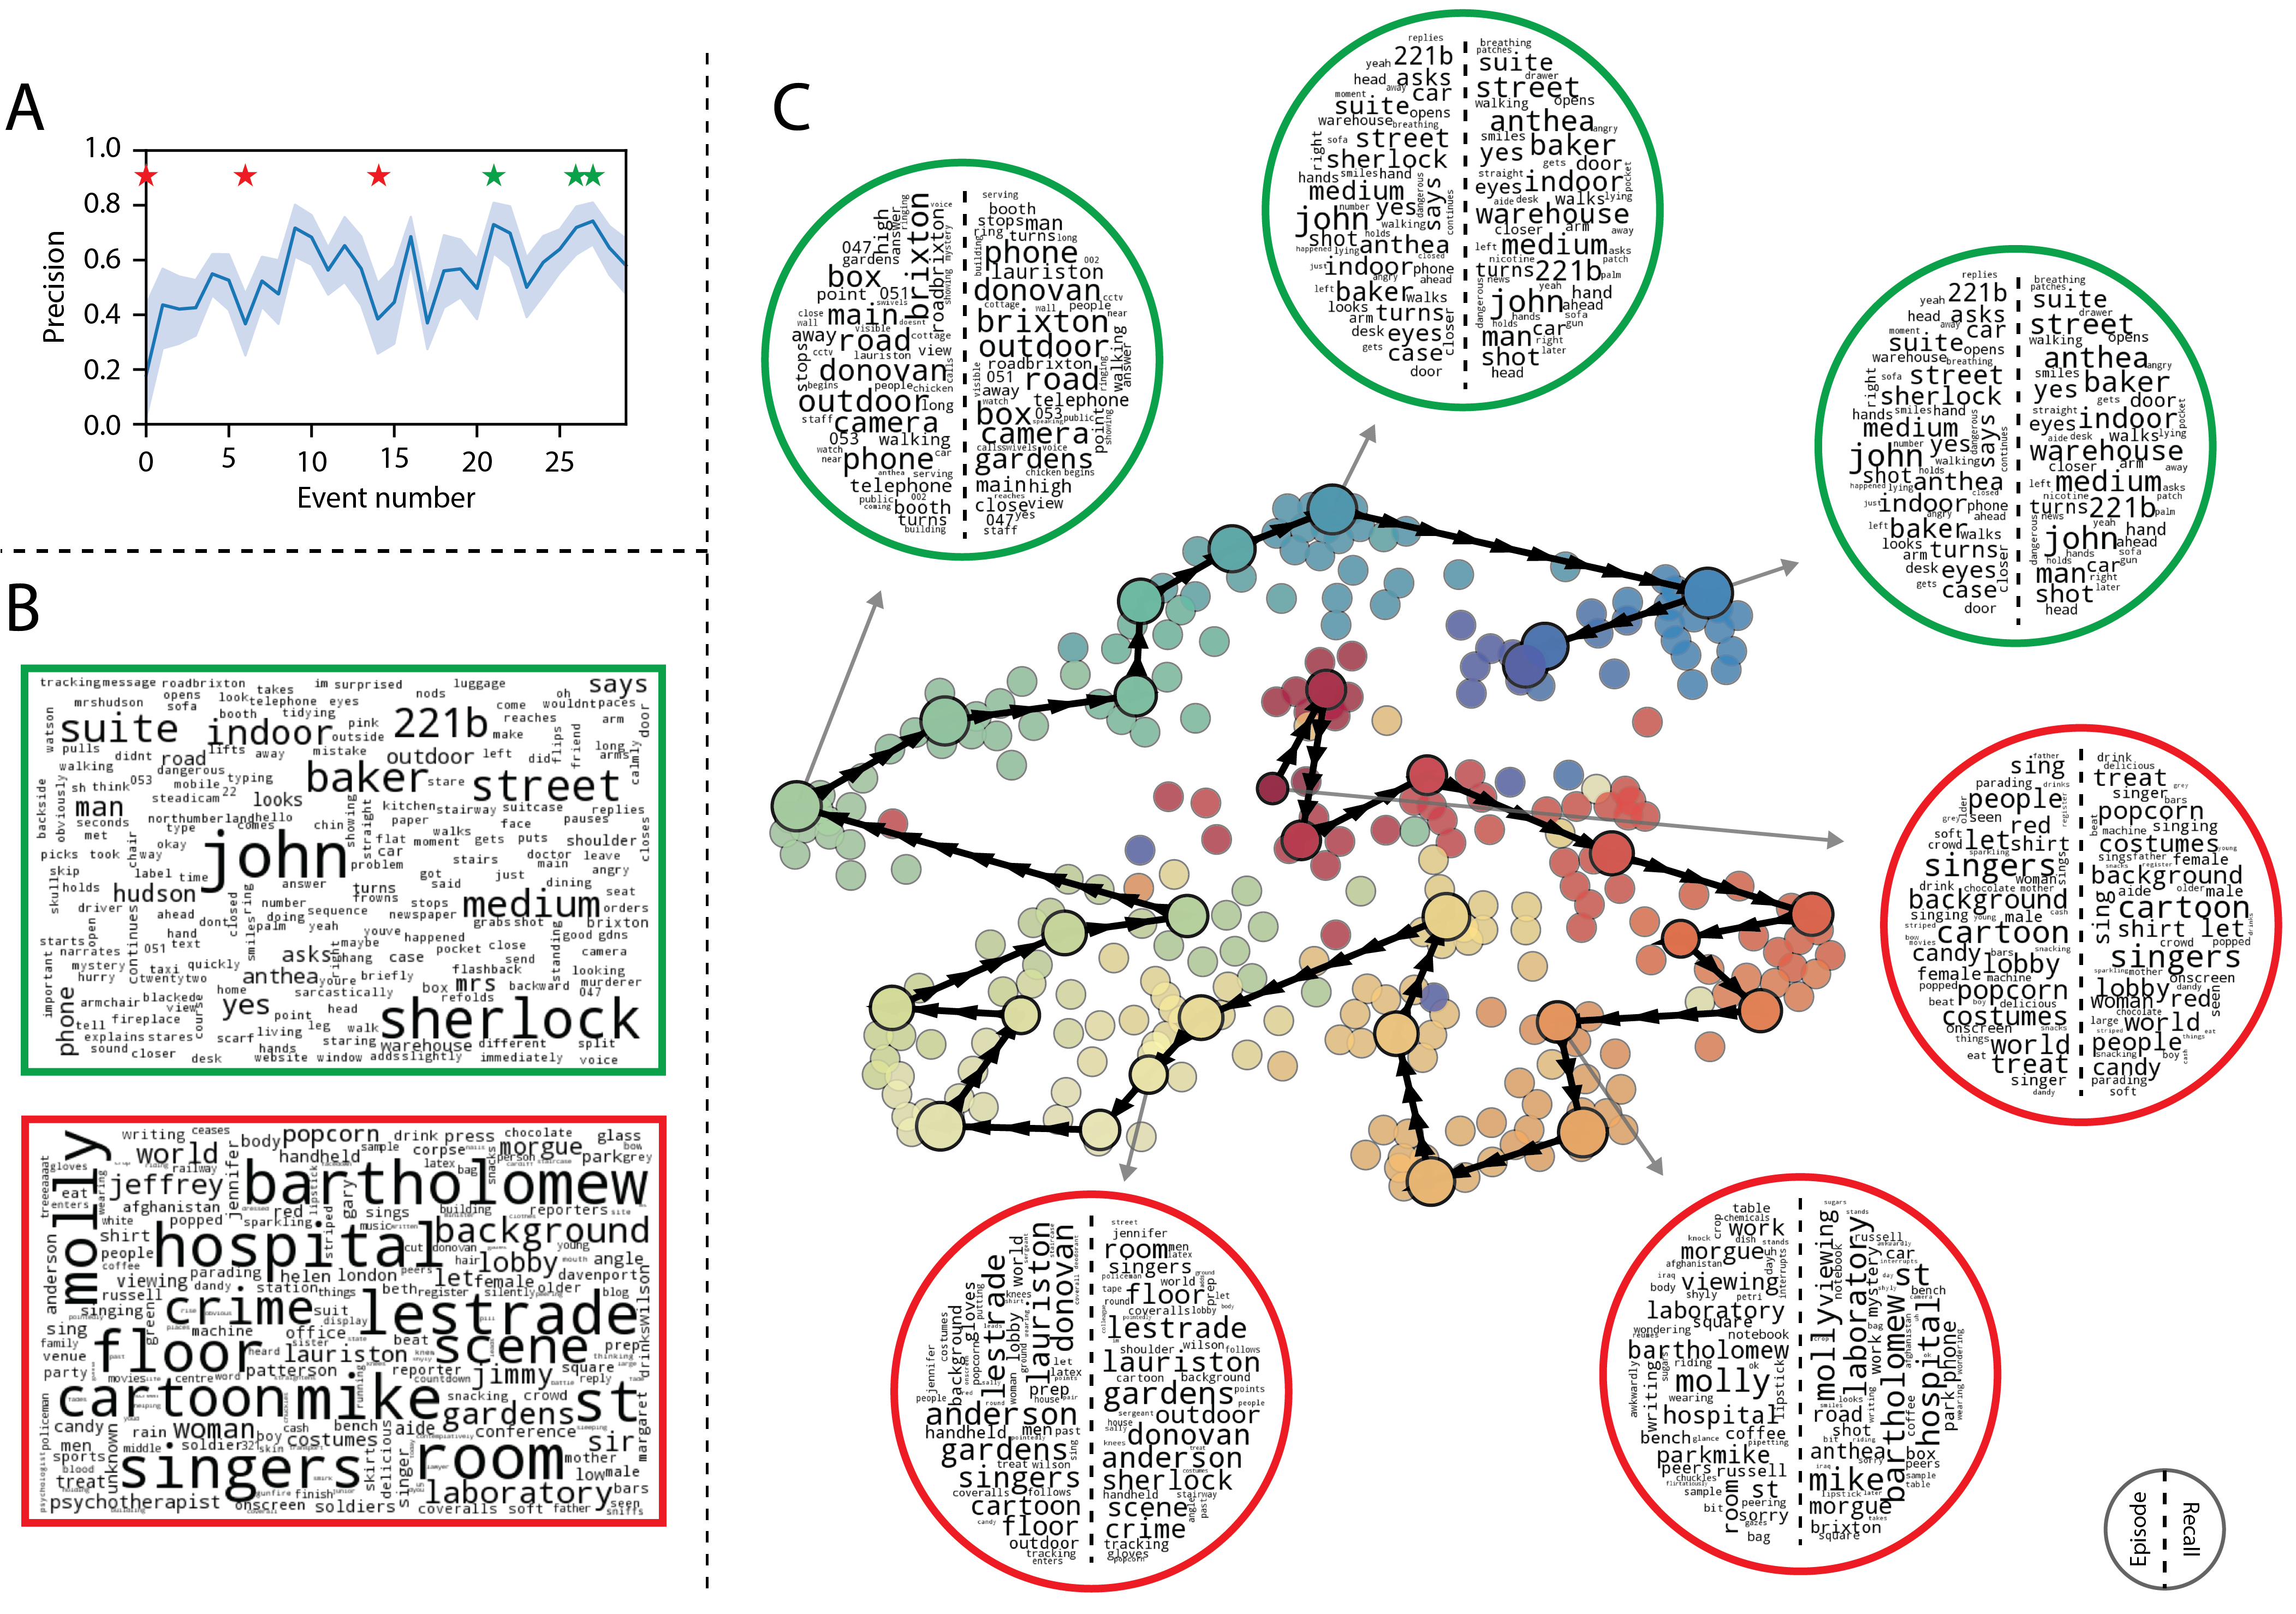
\includegraphics[width=1\textwidth]{figs/topics}
\caption{\small \textbf{Transforming experience into memory.} \textbf{A.} Average correlations (across participants) between the topic vectors from each video event and the closest-matching recall events.  Error bars denote bootstrap-derived across-participant 95\% confidence intervals.  The stars denote the three best-remembered events (green) and worst-remembered events (red).  \textbf{B.} Wordles comprising the top 200 highest-weighted words reflected in the weighted-average topic vector across video events.  Green: video events were weighted by how well the topic vectors derived from recalls of those events matched the video events' topic vectors (Panel A).  Red: video events were weighted by the inverse of how well their topic vectors matched the recalled topic vectors.  \textbf{C.}  The set of all video and recall events is projected onto the two-dimensional space derived in Figure~\ref{fig:trajectory}.  The dots outlined in black denote video events (dot size reflects the average correlation between the video event's topic vector and the topic vectors from the closest matching recalled events from each participant; bigger dots denote stronger correlations).  The dots without black outlines denote recalled events.  All dots are colored using the same scheme as Figure~\ref{fig:trajectory}A.  Wordles for several example events are displayed (green: three best-remembered events; red: three worst-remembered events).  Within each circular wordle, the left side displays words associated with the topic vector for the video event, and the right side displays words associated with the (average) recall event topic vector, across all recall events matched to the given video event.}
\label{fig:topics}
\end{figure}

The results thus far inform us about which aspects of the dynamic content in the episode participants watched were preserved or altered in participants' memories of the episode.  We next carried out a series of analyses aimed at understanding which brain structures might implement these processes.  In one analysis we sought to identify which brain structures were sensitive to the video's dynamic content, as characterized by its topic trajectory.  Specifically, we used a searchlight procedure to identify the extent to which each cluster of voxels exhibited a timecourse (as the participants watched the video) whose temporal correlation matrix matched the temporal correlation matrix of the original video's topic proportion matrix (Fig.~\ref{fig:model}B).  As shown in Figure~\ref{fig:brainz}A, the analysis revealed a network of regions including bilateral frontal cortex and cingulate cortex, suggesting that these regions may play a role in maintaining information relevant to the narrative structure of the video.  In a second analysis, we sought to identify which brain structures' responses (while viewing the video) reflected how each participant would later \textit{recall} the video.  We used an analogous searchlight procedure to identify clusters of voxels whose temporal correlation matrices reflected the temporal correlation matrix of the topic proportions for each individual's recalls (Figs.~\ref{fig:model}D, \corrmats).  As shown in Figure~\ref{fig:brainz}B, the analysis revealed a network of regions including the ventromedial prefrontal cortex (vmPFC), anterior cingulate cortex, and right medial temporal lobe (rMTL), suggesting that these regions may play a role in transforming each individual's experience into memory.  In identifying regions whose responses to ongoing experiences reflect how those experiences will be remembered later, this latter analysis extends classic \textit{subsequent memory analyses}~\citep[e.g.,][]{PallWagn02} to domain of naturalistic stimuli.

\begin{figure}[tp]
\centering
\includegraphics[width=1\textwidth]{figs/brains_panels}
\caption{\small \textbf{Brain structures that underlie the transformation of experience into memory.} \textbf{A.} We searched for regions whose responses (as participants watched the video) matched the temporal correlation matrix of the video topic proportions.  These regions are sensitive to the narrative structure of the video.  \textbf{B.} We searched for regions whose responses (as participants watched the video) matched the temporal correlation matrix of the topic proportions derived from each individual's later recall of video.  These regions are sensitive to how the narrative structure of the video is transformed into a memory of the video.  Both panels: the maps are thresholded at $p < 0.05$, corrected.}
\label{fig:brainz}
\end{figure}


\section*{Discussion}
\label{sec:discussion}

Our work casts remembering as reproducing (behaviorally and neurally) the topic trajectory, or shape, of the original experience.  This view draws inspiration from prior work aimed at elucidating the neural and behavioral underpinnings of how we process dynamic naturalistic experiences and remember them later.  One approach to identifying neural responses to naturalistic stimuli (including experiences) entails building a model of the stimulus and searching for brain regions whose responses are consistent with the model.  In prior work, a series of studies from Uri Hasson's group~\citep{LernEtal11, SimoEtal16, ChenEtal17, BaldEtal17, ZadbEtal17} have extended this approach with a clever twist.  Rather than building an explicit stimulus model, these studies instead search for brain responses (while experiencing the stimulus) that are reliably similar across individuals.  So called \textit{inter-subject correlation} (ISC) and \textit{inter-subject functional connectivity} (ISFC) analyses effectively treat other people's brain responses to the stimulus as a ``model'' of how its features change over time.  By contrast, in our present work we used topic models and HMMs to construct an explicit stimulus model (i.e., the topic trajectory of the video).  When we searched for brain structures whose responses are consistent with the video's topic trajectory, we identified a network of structures that overlapped strongly with the ``long temporal receptive window'' network reported by the Hasson group~\citep[e.g., compare our Fig.~\ref{fig:brainz}A with the map of long temporal receptive window voxels in][]{LernEtal11}.  This provides support for the notion that part of the long temporal receptive window network may be maintaining an explicit model of the stimulus dynamics.  When we performed a similar analysis after swapping out the video's topic trajectory with the recall topic trajectories of each individual participant, this allowed us to identify brain regions whose responses (as the participants viewed the video) reflected how the video trajectory would be transformed in memory (as reflected by the recall topic trajectories).  The analysis revealed that the rMTL and vmPFC may play a role in this person-specific transformation from experience into memory.  The role of the MTL in episodic memory encoding has been well-reported~\citep[e.g., ][]{PallWagn02, DavaEtAl03, RangEtal04, Dava06}.  Prior work has also implicated the medial prefrontal cortex in representing ``schema'' knowledge~\citep[i.e., general knowledge about the format of an ongoing experience given prior similar experiences; ][]{KestEtal12, SchlPres15, GilbMarl17, SpalEtal18}.  Integrating across our study and this prior work, one interpretation is that the person-specific transformations mediated (or represented) by the rMTL and vmPFC may reflect schema knowledge being leveraged, formed, or updated, incorporating ongoing experience into previously acquired knowledge.

When modeling memory experiments, often times events (or items) and their later memories are treated as binary (or categorical in the case of confidence ratings) and independent events. Our novel framework allows one to assess memory performance in a more continuous way, as well as analyze the correlational structure of each encoding event to each memory event. Further and importantly, it allows for consideration of the actual content of the experience/memories, which is not typically modeled. Leveraging this, using 2 novel memory metrics we find that the successful memory performance is related to 1) the \textit{precision} with which the participant recounts each event and 2) how \textit{distinctive} each recall event is (relative to the other recalled events). The first finding suggests to us that the accuracy of recall for \textit{any individual event} may predict the overall amount of information recovered by the participant.  The second finding suggests that remembering/describing events in a unique way (relative to other recalled events) is also related to the quantity of content recovered. Intriguingly, prior studies show that pattern separation, or the ability to discriminate between similar experiences, is impaired in many cognitive disorders as well as natural aging [Craig Stark and friends].  Future work might explore how/whether these metrics compare between cognitively impoverished groups and healthy controls.

While a large number of language models exist (e.g. WAS, LSA, word2vec, universal sentence encoder), here we use topic models for a few reasons [CITE THESE].  First, topic models capture the \textit{essence} of a text passage devoid of the specific set and order of words used.  This was an important feature of our model since different people may accurately recall a scene using very different language. Secondly, words can mean different things in different contexts (e.g. baseball bat vs. the animal bat), and topic models are robust to this since words can be part of multiple topics.  Lastly, topic models provide a straight forward to recover the weights for the particular words comprising a topic, allowing for easy interpretation of an event's contents (e.g. Fig.~\ref{fig:topics}). Other models such as Google's universal sentence encoder offer a context-sensitive encoding of text passages, but the encoding space is complex and non-linear and thus, recovering the original words used to fit the model is not straight forward.  

However, it's worth pointing out that our framework is divorced from the particular choice of language model. Moreover, many of the aspects of our framework could be swapped out for other choices. For example, the language model, the timeseries segmentation model and the video-recall matching function could all be customized for the particular problem. Indeed for some problems, recovery of the particular recall words may not be necessary, and thus other text-modeling approaches (such as universal sentence encoder) may be preferable. Future work will explore the influence of particular model choices on the framework's accuracy.

Our work has broad implications for how we characterize and assess memory in real-world settings such as the classroom or physician's office.  For example, the most commonly used classroom evaluation tools involve computing the proportion of correctly answered exam questions.  Our work indicates that this approach is only loosely related to what educators might really want to measure: how well did the students understand the key ideas presented in the course?  One could apply the computational framework we developed to construct topic trajectories for the video and participants' recalls to build explicit content models of the course material and exam questions.  This approach would provide a more nuanced and specific view into which aspects of the material students had learned well (or poorly).  In clinical settings, memory measures that incorporate such explicit content models might also provide more direct evaluations of patients' memories.


\section*{Methods}
\label{sec:methods}

\subsection*{Experimental design and data collection}
Data were collected by \cite{ChenEtal17}.  In brief, participants ($n=17$) viewed the first 48 minutes of ``A Study in Pink'', the first episode of the BBC television series \textit{Sherlock}, while fMRI volumes were collected (TR = 1500~ms).  The stimulus was divided into a 23~min (946~TR) and a 25~min (1030~TR) segment to mitigate technical issues related to the scanner.  After finishing the clip, participants were instructed to \citep[quoting from][]{ChenEtal17} ``describe what they recalled of the [episode] in as much detail as they could, to try to recount events in the original order they were viewed in, and to speak for at least 10 minutes if possible but that longer was better. They were told that completeness and detail were more important than temporal order, and that if at any point they realized they had missed something, to return to it. Participants were then allowed to speak for as long as they wished, and verbally indicated when they were finished (e.g., `I’m done').''  For additional details about the experimental procedure and scanning parameters see \cite{ChenEtal17}.  The experimental protocol was approved by Princeton University's Institutional Review Board.

After preprocessing the fMRI data and warping the images into a standard (3~mm$^3$ MNI) space, the voxel activations were $z$-scored (within voxel) and spatially smoothed using a 6~mm (full width at half maximum) Gaussian kernel.  The fMRI data were also cropped so that all video-viewing data were aligned across participants.  This included a constant 3 TR (4.5~s) shift to account for the lag in the hemodynamic response.  \citep[All of these preprocessing steps followed][where additional details may be found.]{ChenEtal17}

\subsection*{Data and code availability}
The fMRI data we analyzed are available online \href{http://dataspace.princeton.edu/jspui/handle/88435/dsp01nz8062179}{\underline{here}}.  The behavioral data and all of our analysis code may be downloaded \href{https://github.com/ContextLab/sherlock-topic-model-paper}{\underline{here}}.

\subsection*{Statistics}
All statistical tests we performed were two-sided.

\subsection*{Modeling the dynamic content of the video and recall transcripts}
\subsubsection*{Topic modeling}
The input to the topic model we trained to characterize the dynamic content of the video comprised hand-generated annotations of each of 1000 scenes spanning the video clip~\citep[generated by][]{ChenEtal17}.  The features included: narrative details (a sentence or two describing what happened in that scene); whether the scene took place indoors or outdoors; names of any characters that appeared in the scene; name(s) of characters in camera focus; name(s) of characters who were speaking in the scene; the location (in the story) that the scene took place; camera angle (close up, medium, long, top, tracking, over the shoulder, etc.); whether music was playing in the scene or not; and a transcription of any on-screen text.  We concatenated the text for all of these features within each segment, creating a ``bag of words'' describing each scene.  We then re-organized the text descriptions into overlapping sliding windows spanning 50 scenes each. In other words, the first text sample comprised the combined text from the first 50 scenes (i.e., 1--50), the second comprised the text from scenes 2--51, and so on.  We trained our model using these overlapping text samples with \texttt{scikit-learn}~\citep[version 0.19.1; ][]{PedrEtal11}, called from our high-dimensional visualization and text analysis software, \texttt{HyperTools}~\citep{HeusEtal18a}.  Specifically, we use the \texttt{CountVectorizer} class to transform the text from each scene into a vector of word counts (using the union of all words across all scenes as the ``vocabulary,'' excluding English stop words); this yields a number-of-scenes by number-of-words \textit{word count} matrix.  We then use the \texttt{LatentDirichletAllocation} class (topics=100, method=`batch') to fit a topic model~\citep{BleiEtal03} to the word count matrix, yielding a number-of-scenes (1000) by number-of-topics (100) \textit{topic proportions} matrix.  The topic proportions matrix describes which mix of topics (latent themes) is present in each scene.  Next, we transformed the topic proportions matrix to match the 1976 fMRI volume acquisition times.  For each fMRI volume, we took the topic proportions from whatever scene was displayed for most of that volume's 1500~ms acquisition time.  This yielded a new number-of-TRs (1976) by number-of-topics (100) topic proportions matrix.

We created similar topic proportions matrices using hand-annotated transcripts of each participant's recall of the video~\citep[annotated by ][]{ChenEtal17}.  We tokenized the transcript into a list of sentences, and then re-organized the list into overlapping sliding windows spanning 10 sentences each; in turn we transformed each window's sentences into a word count vector (using the same vocabulary as for the video model).  We then used the topic model already trained on the video scenes to compute the most probable topic proportions for each sliding window.  This yielded a number-of-sentences (range: 68--294) by number-of-topics (100) topic proportions matrix, for each participant.  These reflected the dynamic content of each participant's recalls.  Note: for details on how we selected the video and recall window lengths and number of topics, see \textit{Supporting Information} and Figure~\topicopt.

\subsubsection*{Parsing topic trajectories into events using Hidden Markov Models}
We parsed the topic trajectories of the video and participants' recalls into events using Hidden Markov Models~\citep{Rabi89}.  Given the topic proportions matrix (describing the mix of topics at each timepoint) and a number of states, $K$, an HMM recovers the set of state transitions that segments the timeseries into $K$ discrete states.  Following \cite{BaldEtal17}, we imposed an additional set of constraints on the discovered state transitions that ensured that each state was encountered exactly once (i.e., never repeated).  We used the BrainIAK toolbox~\citep{Brainiak} to implement this segmentation.

We used an optimization procedure to select the appropriate $K$ for each topic proportions matrix.  Specifically, we computed (for each matrix)
\[
  \argmax_K \left[\frac{a}{b} - \frac{K}{\alpha}\right],
\]
where $a$ was the average correlation between the topic vectors of timepoints within the same state; $b$ was the average correlation between the topic vectors of timepoints within \textit{different} states; and $\alpha$ was a regularization parameter that we set to 5 times the window length (i.e., 250 scenes for the video topic trajectory and 50 sentences for the recall topic trajectories).  Figure~\ref{fig:model}B displays the event boundaries returned for the video, and Figure~\corrmats~displays the event boundaries returned for each participant's recalls.  After obtaining these event boundaries, we created stable estimates of each topic proportions matrix by averaging the topic vectors within each event.  This yielded a number-of-events by number-of-topics matrix for the video and recalls from each participant.

We also evaluated a parameter-free procedure for choosing $K$, which finds the $K$ value that maximizes the Wasserstein distance (a.k.a. "Earth mover's" distance) between the within and across event distributions of correlation values. This alternative procedure largely replicated the pattern of results found with the parameterized method described above, but recovered substantially fewer events on average (Fig.\wasserstein). While both approaches seem to underestimate the number of video/recall events relative to the "true" number (as determined by human raters), the parameterized approach was closer to the true number.


\subsubsection*{Visualizing the video and recall topic trajectories}
We used the UMAP algorithm~\citep{McInHeal18} to project the 100-dimensional topic space onto a two-dimensional space for visualization (Figs.~\ref{fig:trajectory}, \ref{fig:topics}).  To ensure that all of the trajectories were projected onto the \textit{same} lower dimensional space, we computed the low-dimensional embedding on a ``stacked'' matrix created by vertically concatenating the events-by-topics topic proportions matrices for the video and all 17 participants' recalls.  We then divided the rows of the result (a total-number-of-events by two matrix) back into separate matrices for the video topic trajectory and the trajectories for each participant's recalls (Fig.~\ref{fig:trajectory}).  This general approach for discovering a shared low-dimensional embedding for a collections of high-dimensional observations follows \cite{HeusEtal18a}.


\subsubsection*{Estimating the consistency of flow through topic space across participants}
In Figure~\ref{fig:trajectory}B, we present an analysis aimed at characterizing locations in topic space that different participants move through in a consistent way (via their recall topic trajectories).  The two-dimensional topic space used in our visualizations (Fig.~\ref{fig:trajectory}) ranged from -5 to 5 (arbitrary) units in the $x$ dimension and from -6.5 to 2 units in the $y$ dimension.  We divided this space into a grid of vertices spaced 0.25~units apart.  For each vertex, we examined the set of line segments formed by connecting each pair successively recalled events, across all participants, that passed within 0.5 units.  We computed the distribution of angles formed by those segments and the $x$-axis, and used a Rayleigh test to determine whether the distribution of angles was reliably ``peaked'' (i.e., consistent across all transitions that passed through that local portion of topic space).  To create Figure~\ref{fig:trajectory}B we drew an arrow originating from each grid vertex, pointing in the direction of the average angle formed by line segments that passed within 0.5 units.  We set the arrow lengths to be inversely proportional to the $p$-values of the Rayleigh tests at each vertex.  Specifically, for each vertex we converted all of the angles of segments that passed within 0.5 units to unit vectors, and we set the arrow lengths at each vertex proportional to the length of the (circular) mean vector.  We also indicated any significant results ($p < 0.05$, corrected using the Benjamani-Hochberg procedure) by coloring the arrows in blue (darker blue denotes a lower $p$-value, i.e., a longer mean vector); all tests with $p \geq 0.05$ are displayed in gray and given a lower opacity value.

\subsection*{Naturalistic extensions of classic list-learning analyses}
In traditional list-learning experiments, participants view a list of items (e.g., words) and then recall the items later.  Our video-recall event matching approach affords us the ability to analyze memory in a similar way. The video and recall events can be treated analogously to studied and recalled ``items'' in a list-learning study.  We can then extend classic analyses of memory performance and dynamics (originally designed for list-learning experiments) to the more naturalistic video recall task used in our study.

Perhaps the simplest and most widely used measure of memory performance is \textit{accuracy}-- i.e., the proportion of studied (experienced) items (in this case, the 34 video events) that the participant later remembered.  \cite{ChenEtal17} developed a human rating system whereby the quality of each participant's memory was evaluated by an independent rater.  We found a strong across-participants correlation between these independant ratings and the overall number of events that our HMM approach identified in participants' recalls (Pearson's $r(15) = 0.67, p = 0.003$).

As described below, we next considered a number of memory performance measures that are typically associated with list-learning studies.  We also provide a software package, \texttt{Quail}, for carrying out these analyses~\citep{HeusEtal17b}.

\paragraph{Probability of first recall (PFR).}  PFR curves~\citep{WelcBurn24, PostPhil65, AtkiShif68} reflect the probability that an item will be recalled first as a function of its serial position during encoding. To carry out this analysis, we initialized a number-of-participants (17) by number-of-video-events (34) matrix of zeros. Then for each participant, we found the index of the video event that was recalled first (i.e., the video event whose topic vector was most strongly correlated with that of the first recall event) and filled in that index in the matrix with a 1.  Finally, we averaged over the rows of the matrix, resulting in a 1 by 34 array representing the proportion of participants that recalled an event first, as a function of the order of the event's appearance in the video (Fig.~\ref{fig:list-learning}A).

\paragraph{Lag conditional probability curve (lag-CRP).} The lag-CRP curve~\citep{Kaha96} reflects the probability of recalling a given event after the just-recalled event, as a function of their relative positions (or \textit{lag}).  In other words, a lag of 1 indicates that a recalled event came immediately after the previously recalled event in the video, and a lag of -3 indicates that a recalled event came 3 events before the previously recalled event.  For each recall transition (following the first recall), we computed the lag between the current recall event and the next recall event, normalizing by the total number of possible transitions.  This yielded a number-of-participants (17) by number-of-lags (-33 to +33; 67 lags total) matrix. We averaged over the rows of this matrix to obtain a group-averaged lag-CRP curve (Fig.~\ref{fig:list-learning}B).

\paragraph{Serial position curve (SPC).} SPCs~\citep{Murd62a} reflect the proportion of participants that remember each item as a function of their serial position during encoding. We initialized a number-of-participants (17) by number-of-video-events (34) matrix of zeros. Then, for each recalled event, for each participant, we found the index of the video event that the recalled event most closely matched (via the correlation between the events' topic vectors) and entered a 1 into that position in the matrix (i.e., for the given participant and event). This resulted in a matrix whose entries indicated whether or not each event was recalled by each participant (depending on whether the corresponding entires were set to one or zero).  Finally, we averaged over the rows of the matrix to yield a 1 by 34 array representing the proportion of participants that recalled each event as a function of the order of the event's appearance in the video (Fig.~\ref{fig:list-learning}C).

\paragraph{Temporal clustering scores.} Temporal clustering refers to the extent to which participants group their recall responses according to encoding position~\citep{PolyEtal09}. For instance, if a participant recalled the video events in the exact order they occurred (or in exact reverse order), this would yield a score of 1.  If a participant recalled the events in random order, this would yield an expected score of 0.5.  For each recall event transition (and separately for each participant), we sorted all not-yet-recalled events according to their absolute lag (i.e., distance away in the video).  We then computed the percentile rank of the next event the participant recalled.  We averaged these percentile ranks across all of the participant's recalls to obtain a single temporal clustering score for the participant (mean: 0.808, SEM: 0.022).  Overall, we found that participants with higher temporal clustering scores also tended to recall more events (Pearson's $r(15) = 0.62, p = 0.007$).

\paragraph{Semantic clustering scores.} Semantic clustering measures the extent to which participants clustered their recall responses according to semantic similarity~\citep{PolyEtal09}. Here, we used the topic vectors for each event as a proxy for its semantic content. Thus, the similarity between the semantic content for two events can be computed by correlating their respective topic vectors.  For each recall event transition, we sorted all not-yet-recalled events according to how correlated the topic vector \textit{of the closest-matching video event} was to the topic vector of the closest-matching video event to the just-recalled event.  We then computed the percentile rank of the observed next recall.  We averaged these percentile ranks across all of the participant's recalls to obtain a single semantic clustering score for the participant (mean: 0.813, SEM: 0.022).  We found that participants who exhibited stronger semantic clustering scores overall remembered more video events (Pearson's $r(15) = 0.55, p = 0.02$).


% NOTE: Thinking about removing this analysis? More of a sanity check than something novel and cool, and takes up space. Happy to be convinced otherwise

% To quantify the similarity between the video topic trajectory and individual recall topic trajectories, we considered several novel metrics.  First, we tested whether each participant's recall trajectory matched the video trajectory in a general sense. For each participant we filtered the video trajectory to only include the events that the participant remembered.  We then computed the root mean squared difference (RMSD) between the remaining video events and the (closest-matching) recalled events.  For example, if the topic vectors for a participant's recall event topic vectors matched the corresponding video event topic vectors exactly (and in order), the expected RMSD for those events would be 0.  However, if the participant's recall events did not perfectly match the video events, or if they were out of order, then the RMSD would be greater than 0.  To assess the significance of the match between the video and recall trajectories, we carried out a permutation procedure whereby, for each of 10000 repetitions, we circularly shifted the recall trajectories (in time) by a random amount and then re-computed the RMSD each time.  This yielded a distribution of ``null'' RMSD values for each participant.  The observed RMSD values reached significance (i.e., $p < 0.05$, reflecting that more than 95\% of the null RMSD values were greater than the observed RMSD value) for nine of the participants (3, 4, 8--13, and 17).  (For the remaining participants this test yielded $0.05 \leq p < 0.25$.)  The observed RMSD values were also reliably correlated with hand-annotated memory performance across participants (Pearson's $r(15) = -0.57, p = 0.016$).  In other words, a closer match between the video and recall topic trajectories was related to better overall recall performance.

\paragraph*{Precision.}
We tested whether participants who recalled more events were also more \textit{precise} in their recollections. For each participant, we computed the correlation between the topic vectors for each recall event and that of its closest-matching video event (only for the events which they recalled). We Fisher's z-transformed the correlations, computed the average and then inverse Fisher's z-transformed the resulting value.  This gave a single value per participant representing the average precision across all recalled events.  We then correlated this value with hand-annotated as well as model derived (e.g. $k$ or the number of events recovered by the HMM) memory performance.

\paragraph*{Distinctiveness.}
We also considered the \textit{distinctiveness} of each recalled event. That is, how uniquely a recalled event's topic vector matched a given video event topic vector, versus the topic vectors for the other video events. We hypothesized that participants with high memory performance might describe each event in a more distinctive way (relative to those with lower memory performance who might describe events in a more general way).  To test this hypothesis we define a distinctiveness score for each recalled event as

%NOTE: Need to check on this equation!
\[
  d(\mathrm{event}) = 1 - \bar{c}(\mathrm{event}),
\]
where $\bar{c}(\mathrm{event})$ is the average correlation between the given recalled event's topic vector and the topic vectors from all video events \textit{except} the best-matching video event.  We then averaged these distinctiveness scores across all of the events recalled by the given participant. As above, we used Fisher's z (transform and inverse-transform) before/after averaging correlation values. Finally, we correlated these values with hand-annotated and model derived memory performance scores across-subjects.

\subsection*{Searchlight fMRI analyses}
In Figure~\ref{fig:brainz}, we present two analyses aimed at identifying brain structures whose responses (as participants viewed the video) exhibited particular temporal correlations.  We developed a searchlight analysis whereby we constructed a cube centered on each voxel (radius: 5~voxels).  For each of these cubes, we computed the temporal correlation matrix of the voxel responses during video viewing.  Specifically, for each of the 1976 volumes collected during video viewing, we correlated the activity patterns in the given cube with the activity patterns (in the same cube) collected during every other timepoint.  This yielded a 1976 by 1976 correlation matrix for each cube.

Next, we constructed two sets of ``template'' matrices: one reflected the video's topic trajectory and the other reflected each participant's recall topic trajectory.  To construct the video template, we computed the correlations between the topic proportions estimated for every pair of TRs (prior to segmenting the trajectory into discrete events; i.e., the correlation matrix shown in Figs.~\ref{fig:model}B and \ref{fig:brainz}A).  We constructed similar temporal correlation matrices for each participant's recall topic trajectory (Figs.~\ref{fig:model}D, \corrmats).  However, to correct for length differences and potential non-linear transformations between viewing time and recall time, we first used dynamic time warping~\citep{BernClif94} to temporally align participants' recall topic trajectories with the video topic trajectory (an example correlation matrix before and after warping is shown in Fig.~\ref{fig:brainz}B).  This yielded a 1976 by 1976 correlation matrix for the video template and for each participant's recall template.

To determine which (cubes of) voxel responses reliably matched the video template, we correlated the upper triangle of the voxel correlation matrix for each cube with the upper triangle of the video template matrix~\citep{KrieEtal08b}.  This yielded, for each participant, a single correlation value.  We computed the average (Fisher $z$-transformed) correlation coefficient across participants.  We used a permutation-based procedure to assess significance, whereby we re-computed the average correlations for each of 100 ``null'' video templates (constructed by circularly shifting the template by a random number of timepoints).  (For each permutation, the same shift was used for all participants.)  We then estimated a $p$-value by computing the proportion of shifted correlations that were larger than the observed (unshifted) correlation.  To create the map in Figure~\ref{fig:brainz}A we thresholded out any voxels whose correlation values fell below the 95\textsuperscript{th} percentile of the permutation-derived null distribution.

We used a similar procedure to identify which voxels' responses reflected the recall templates.  For each participant, we correlated the upper triangle of the correlation matrix for each cube of voxels with their (time warped) recall correlation matrix.  As in the video template analysis this yielded a single correlation coefficient for each participant.  However, whereas the video analysis compared every participant's responses to the same template, here the recall templates were unique for each participant.  We computed the average $z$-transformed correlation coefficient across participants, and used the same permutation procedure we developed for the video responses to assess significant correlations.  To create the map in Figure~\ref{fig:brainz}B we thresholded out any voxels whose correlation values fell below the 95\textsuperscript{th} percentile of the permutation-derived null distribution.

\bibliography{memlab}

\section*{Supporting information}
Supporting information is available in the online version of the paper.

\section*{Acknowledgements}
We thank Luke Chang, Janice Chen, Chris Honey, Lucy Owen, Emily Whitaker, and Kirsten Ziman for feedback and scientific discussions. We also thank Janice Chen, Yuan Chang Leong, Kenneth Norman, and Uri Hasson for sharing the data used in our study.  Our work was supported in part by NSF EPSCoR Award Number 1632738. The content is solely the responsibility of the authors and does not necessarily represent the official views of our supporting organizations.

\section*{Author contributions}
Conceptualization: A.C.H. and J.R.M.; Methodology: A.C.H. and J.R.M.; Software: A.C.H., P.C.F. and J.R.M.; Analysis: A.C.H., P.C.F. and J.R.M.; Writing, Reviewing, and Editing: A.C.H., P.C.F. and J.R.M.; Supervision: J.R.M.

\section*{Author information}
The authors declare no competing financial interests.  Correspondence and requests for materials should be addressed to J.R.M. (jeremy.r.manning@dartmouth.edu).


\end{document}
